\chapter{Analyse du taux de réussite au bac}
\section{Introduction}

\section{Analyse de globale} 
\subsection{Évolution du nombre d'inscrits, présents et admis}

\begin{figure}[h]
\centering
\caption{Évolution du nombre d'inscrits, présents et admis au bac (2006-2024)}
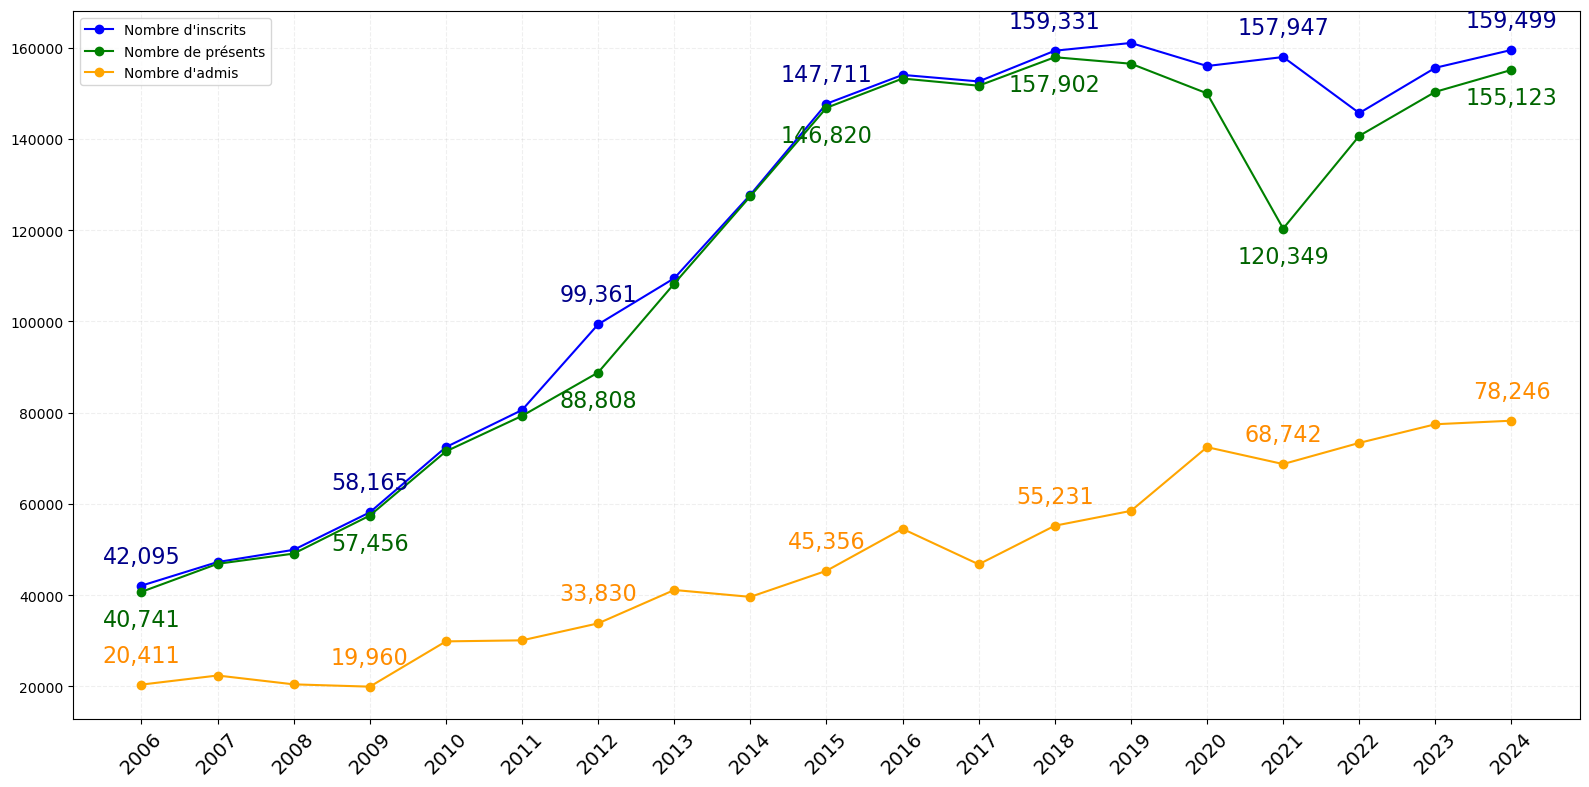
\includegraphics[width=1\textwidth]{figure/Inscrits_bac.png}
\end{figure}

\subsection{Évolution du taux de réussite}

\begin{figure}[h]
\centering
\caption{Évolution du taux de réussite au bac (2006-2024)}
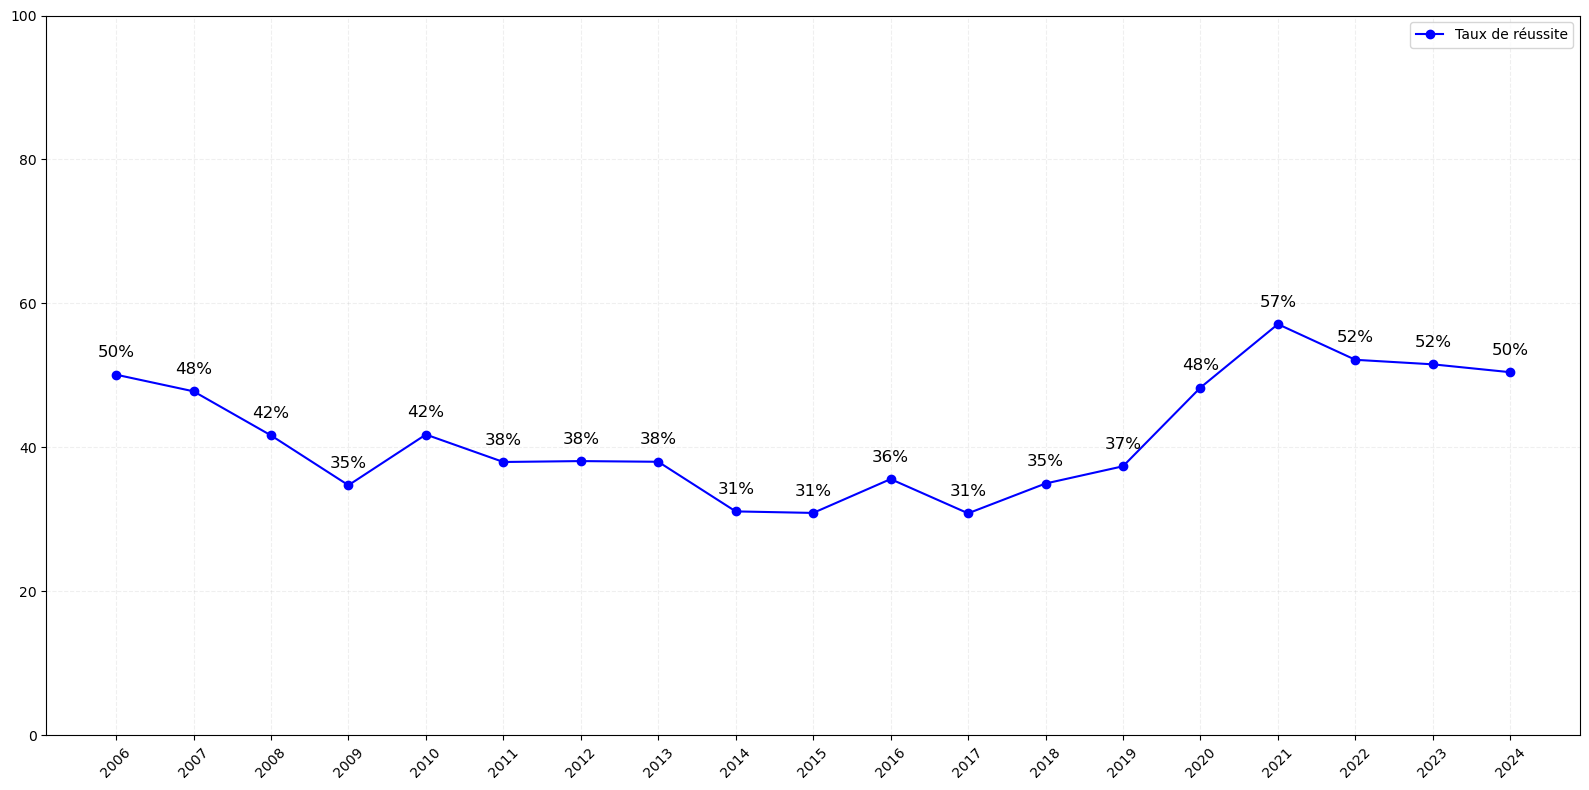
\includegraphics[width=1\textwidth]{figure/taux_bac.png}
\end{figure}

\section{Analyse de la transition entre les séries G et STEG}

\subsection{Évolution du nombre d'inscrits dans les séries G et STEG}

\begin{figure}[h]
\centering
\caption{Évolution du nombre d'inscrits dans les séries G et STEG (2006-2024)}
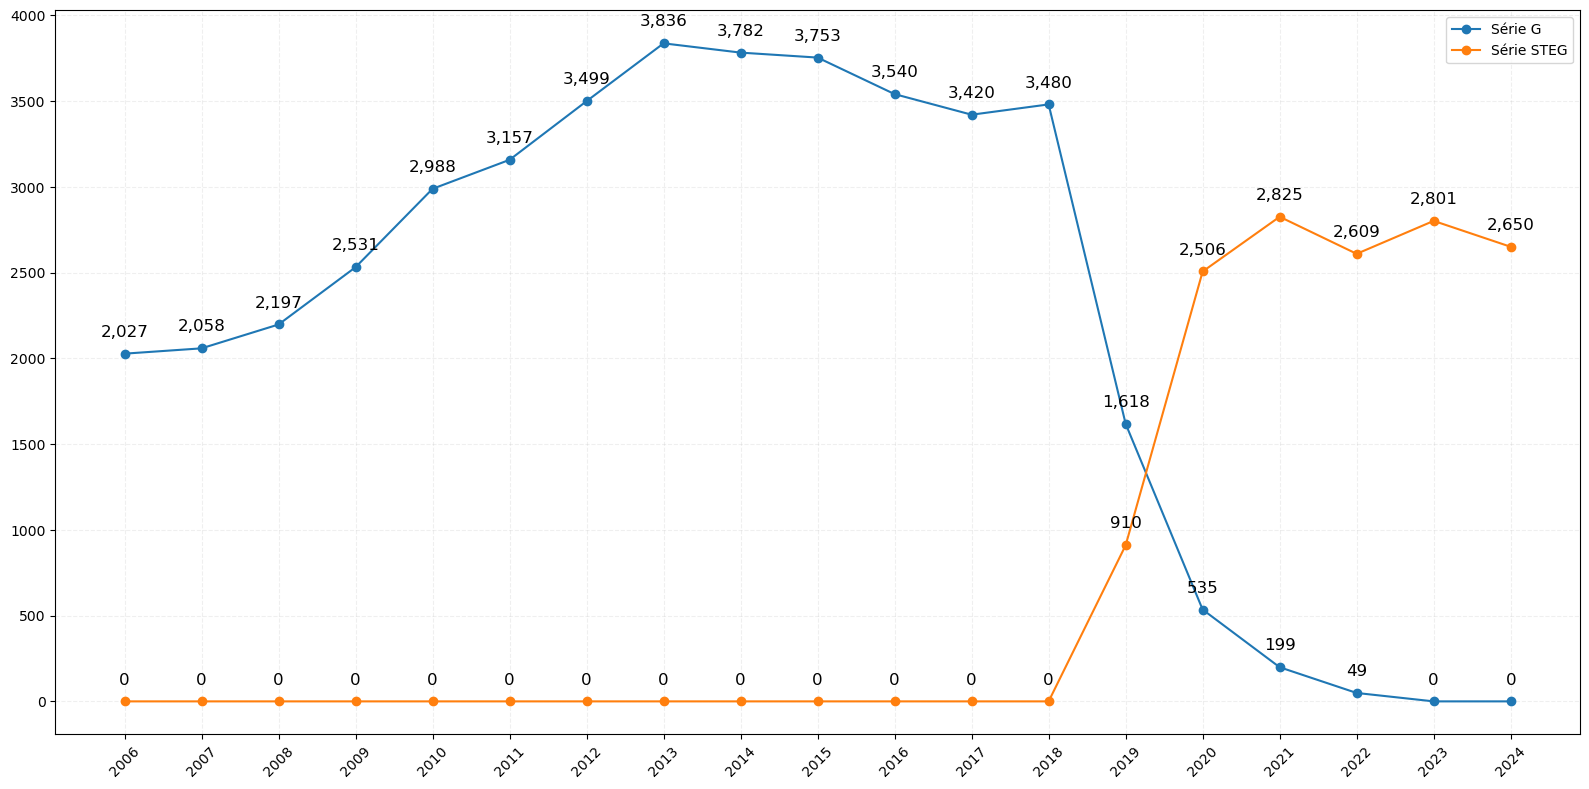
\includegraphics[width=1\textwidth]{figure/Inscrits_bac_STEG.png}
\end{figure}

\subsection{Évolution du taux de réussite dans les séries G et STEG}

\begin{figure}[h]
\centering
\caption{Évolution du taux de réussite dans les séries G et STEG (2006-2024)}
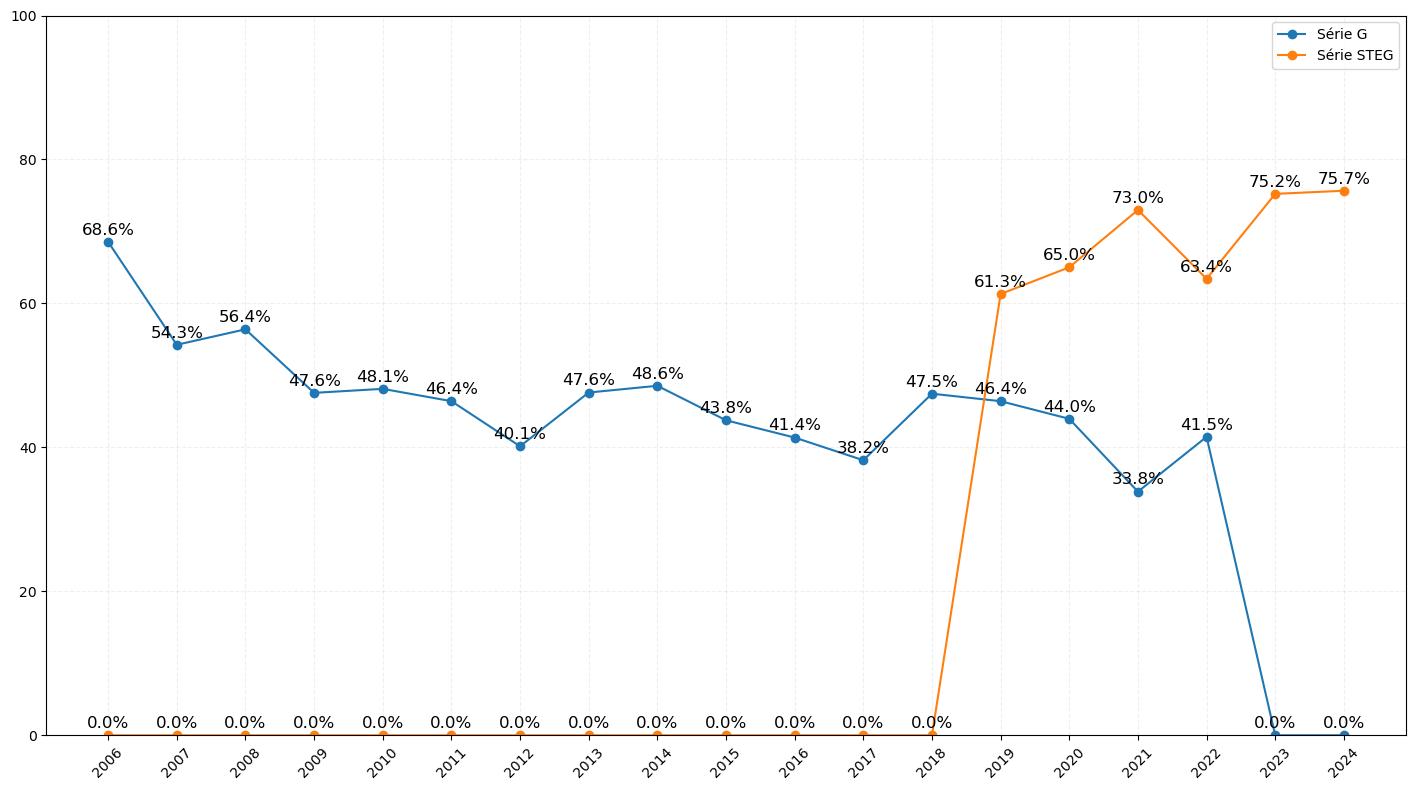
\includegraphics[width=1\textwidth]{figure/taux_bac_STEG.png}
\end{figure}

\newpage
\section{analyse des séries Arabes et Franco-Arabes}

\subsection{Série LA et LAR}

\begin{figure}[h]
\centering
\caption{Évolution du nombre d'inscrits et du taux de réussite dans les séries LA et LAR (2006-2024)}
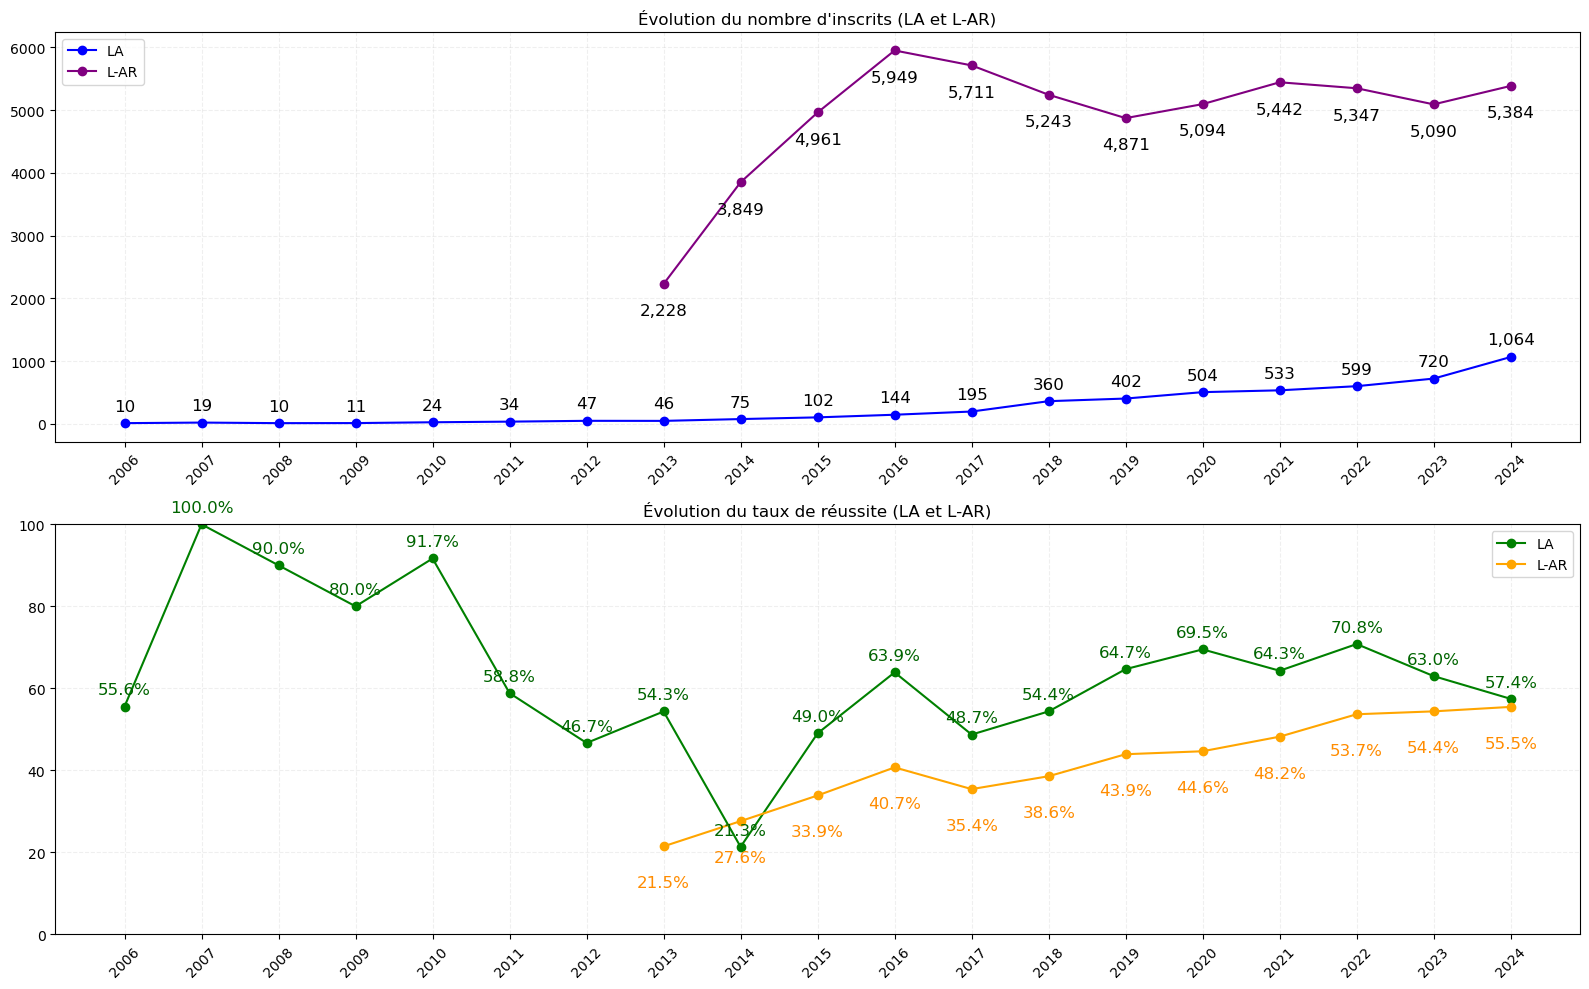
\includegraphics[width=1\textwidth]{figure/bac_LA_LAR.png}
\end{figure}

\newpage
\subsection{Série S2A}

\begin{figure}[h]
\centering
\caption{Évolution du nombre d'inscrits et du taux de réussite dans la série S2A (2006-2024)}
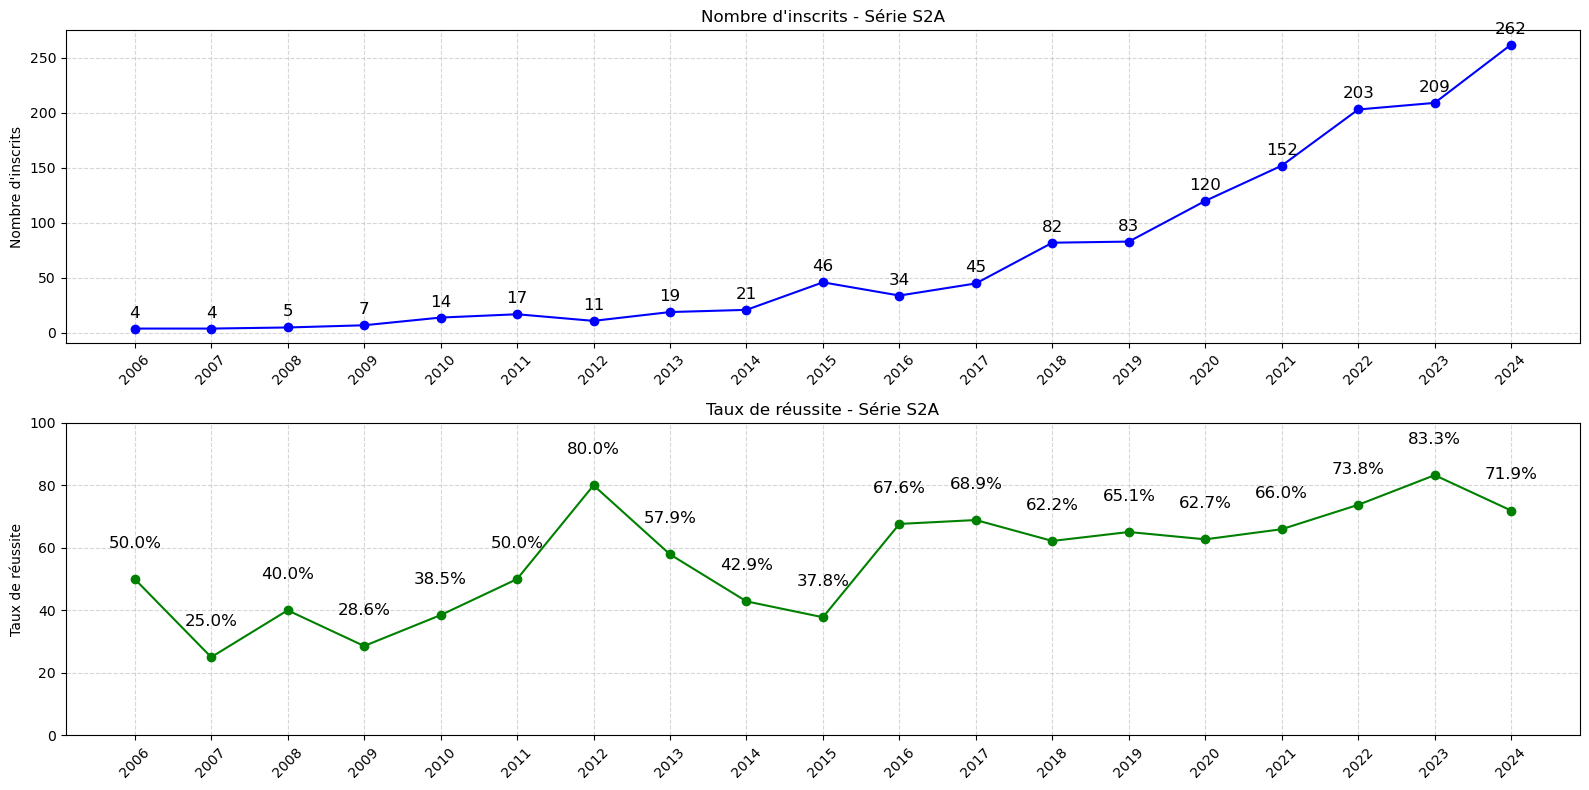
\includegraphics[width=1\textwidth]{figure/bac_S2A.png}
\end{figure}

\newpage
\subsection{Série S2A}

\begin{figure}[h]
\centering
\caption{Évolution du nombre d'inscrits et du taux de réussite dans la série S2A (2006-2024)}
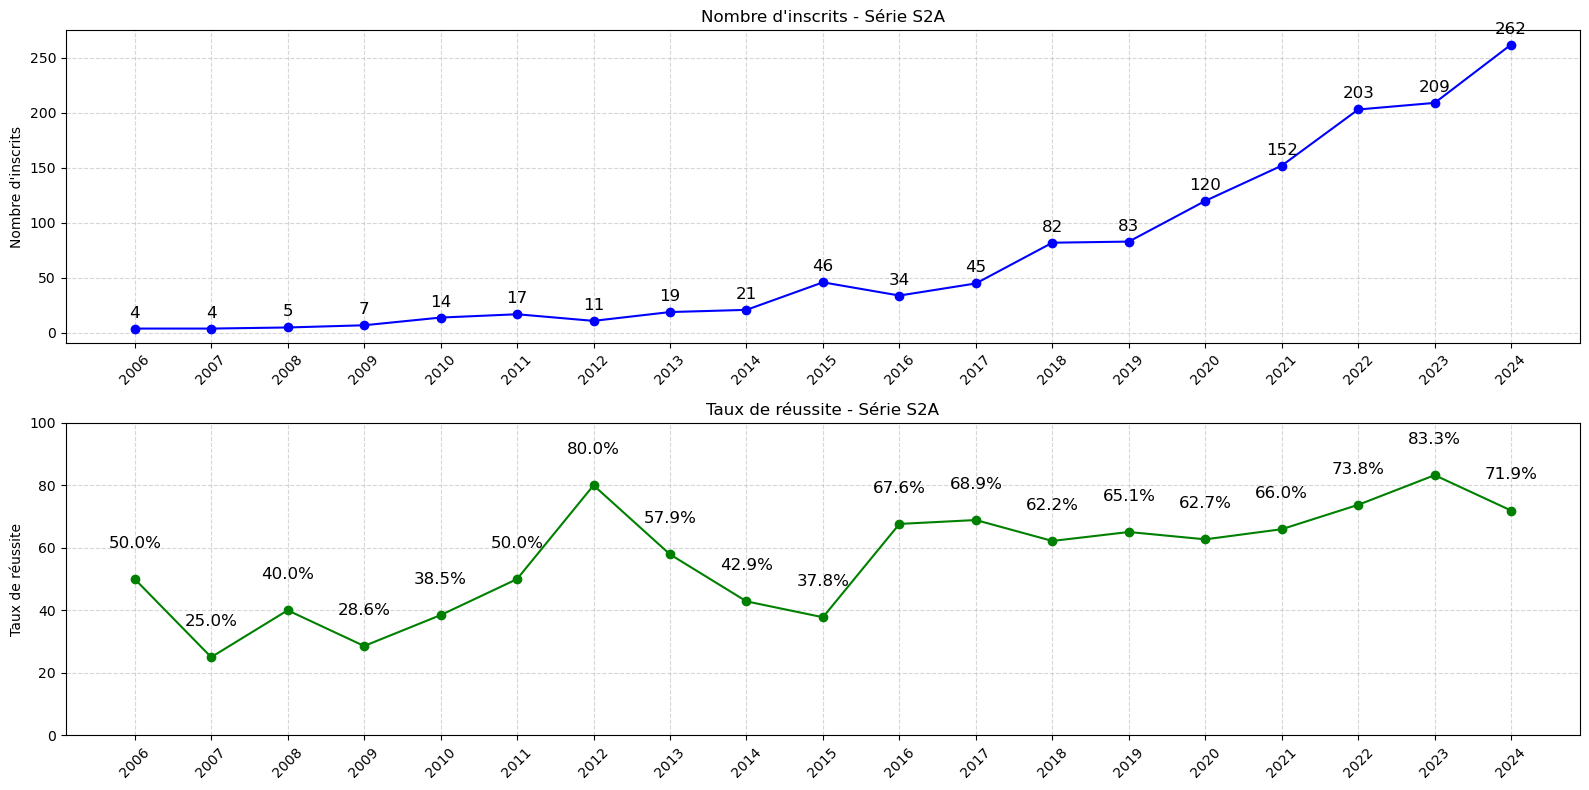
\includegraphics[width=1\textwidth]{figure/bac_S2A.png}
\end{figure}

\newpage
\section{prédiction du taux de réussite}

\section{Conclusion}